


\documentclass{article}\usepackage[]{graphicx}\usepackage[]{color}
%% maxwidth is the original width if it is less than linewidth
%% otherwise use linewidth (to make sure the graphics do not exceed the margin)
\makeatletter
\def\maxwidth{ %
  \ifdim\Gin@nat@width>\linewidth
    \linewidth
  \else
    \Gin@nat@width
  \fi
}
\makeatother

\definecolor{fgcolor}{rgb}{0.2, 0.2, 0.2}
\newcommand{\hlnumber}[1]{\textcolor[rgb]{0,0,0}{#1}}%
\newcommand{\hlfunctioncall}[1]{\textcolor[rgb]{0.501960784313725,0,0.329411764705882}{\textbf{#1}}}%
\newcommand{\hlstring}[1]{\textcolor[rgb]{0.6,0.6,1}{#1}}%
\newcommand{\hlkeyword}[1]{\textcolor[rgb]{0,0,0}{\textbf{#1}}}%
\newcommand{\hlargument}[1]{\textcolor[rgb]{0.690196078431373,0.250980392156863,0.0196078431372549}{#1}}%
\newcommand{\hlcomment}[1]{\textcolor[rgb]{0.180392156862745,0.6,0.341176470588235}{#1}}%
\newcommand{\hlroxygencomment}[1]{\textcolor[rgb]{0.43921568627451,0.47843137254902,0.701960784313725}{#1}}%
\newcommand{\hlformalargs}[1]{\textcolor[rgb]{0.690196078431373,0.250980392156863,0.0196078431372549}{#1}}%
\newcommand{\hleqformalargs}[1]{\textcolor[rgb]{0.690196078431373,0.250980392156863,0.0196078431372549}{#1}}%
\newcommand{\hlassignement}[1]{\textcolor[rgb]{0,0,0}{\textbf{#1}}}%
\newcommand{\hlpackage}[1]{\textcolor[rgb]{0.588235294117647,0.709803921568627,0.145098039215686}{#1}}%
\newcommand{\hlslot}[1]{\textit{#1}}%
\newcommand{\hlsymbol}[1]{\textcolor[rgb]{0,0,0}{#1}}%
\newcommand{\hlprompt}[1]{\textcolor[rgb]{0.2,0.2,0.2}{#1}}%

\usepackage{framed}
\makeatletter
\newenvironment{kframe}{%
 \def\at@end@of@kframe{}%
 \ifinner\ifhmode%
  \def\at@end@of@kframe{\end{minipage}}%
  \begin{minipage}{\columnwidth}%
 \fi\fi%
 \def\FrameCommand##1{\hskip\@totalleftmargin \hskip-\fboxsep
 \colorbox{shadecolor}{##1}\hskip-\fboxsep
     % There is no \\@totalrightmargin, so:
     \hskip-\linewidth \hskip-\@totalleftmargin \hskip\columnwidth}%
 \MakeFramed {\advance\hsize-\width
   \@totalleftmargin\z@ \linewidth\hsize
   \@setminipage}}%
 {\par\unskip\endMakeFramed%
 \at@end@of@kframe}
\makeatother

\definecolor{shadecolor}{rgb}{.97, .97, .97}
\definecolor{messagecolor}{rgb}{0, 0, 0}
\definecolor{warningcolor}{rgb}{1, 0, 1}
\definecolor{errorcolor}{rgb}{1, 0, 0}
\newenvironment{knitrout}{}{} % an empty environment to be redefined in TeX

\usepackage{alltt}
\usepackage{authblk}
\usepackage{caption}
\usepackage{graphicx}
\usepackage{subfig}
\usepackage{pdflscape}
\usepackage{multicol}

\author[1]{Nathan E. Rutenbeck}
\author[2]{Brent R. Frey}
\author[3]{Graeme P. Berlyn}
\author[3]{Oswald J. Schmitz}
\author[4]{Bruce C. Larson}
\author[3]{Mark S. Ashton}
\renewcommand{\Affilfont}{\itshape\small}
\affil[1]{University of Maine, School of Forest Resources, Orono, Maine}
\affil[2]{Department of Forestry, Mississippi State University, MS}
\affil[3]{Yale University, School of Forestry and Environmental Studies, New Haven, CT}
\affil[4]{Faculty of Forestry, University of British Columbia Vancouver, BC, Canada}

\title{Influence of gap position and site preparation on gas exchange dynamics and leaf area of \textit{Picea glauca} and \textit{Populus tremuloides} seedlings in mixedwood stands, Saskatchewan, Canada}
\date{}
\IfFileExists{upquote.sty}{\usepackage{upquote}}{}

\begin{document}\sloppy
\maketitle
\begin{abstract}
\noindent One challenge for managers of boreal and sub-boreal mixedwood stands is to successfully establish and maintain the competitive status of white spruce (\textit{Picea glauca} (Moench) Voss in relation to aspen (\textit{Populus tremuloides} Michx.) and other competitors following harvesting. Underplanting spruce within harvest gaps has been suggested as one potential strategy, but questions remain regarding  the kind of harvest gap environment most conducive to the growth of spruce in relation to aspen. We used linear mixed-effects models to test the effect of harvest gap position and Meri-crusher versus brush-saw vegetation treatment on leaf area per wet weight, leaf photosynthesis, stomatal conductance, and transpiration in low- and full-light conditions, and on photosynthetic plasticity. Overall aspen maintained higher leaf area per unit wet weight than spruce across the gap, but spruce leaf area was more sensitive to changes in gap position. Aspen also maintained higher photosynthesis and transpiration rates than spruce under both light conditions and in both vegetation treatments, but the magnitude of difference in gas exchange rates between the two species depended significantly on vegetation treatment and gap position for photosynthesis, and on gap position for transpiration. Plasticity of photosynthetic response to changes in light were not significantly different for both species, and did not vary significantly with experimental treatments.
\end{abstract}

\begin{multicols}{2}
\section{Introdution}
Throughout the North American boreal and sub-boreal forests a natural disturbance regime of relatively frequent catastrophic fires (Armstrong 1999) facilitates the occurrence of trembling aspen (\textit{Populus tremuloides} Michx.) and white spruce (\textit{Picea glauca} (Moench) Voss) in both single- and stratified mixed-species stands (Rowe 1972, MacLaughlan et al. 2010). On mixedwood sites of this region, aspen is an early-successional pioneer, dominating during stand initiation and stem exclusion phases of stand development (sensu Oliver and Larson 1996). Following fire events, aspen typically regenerates quickly through vigorous root suckering to form a dense, closed canopy within about five years (Frey et al. 2002, Bokalo et al. 2007). Initial colonization by aspen is then followed by a period of intense competition and self-thinning before maturity at around 60-80 years, at which point the aspen component of the stand begins to decline. White spruce can enter these stands via two principal pathways. Spruce can establish via initial floristics, colonizing immediately following disturbance alongside aspen or it can establish later in stand development with the formation of canopy gaps (Dix and Swan 1971, Rowe and Scotter 1973, DeLong 1991, Youngblood 1995, Lieffers et al. 2002). In either case, on mixedwood sites growth of the more shade-tolerant spruce typically lags behind that of the more intolerant aspen, with the spruce component occupying the lower strata beneath aspen for several decades until releasing disturbance events (Nienstadt and Zasada 1990, Peterson and Peterson 1992, Lieffers et al. 1996, Brais et al. 2004).

Because of the economic value of white spruce, however, managers of these forests often seek to generate spruce volumes on a shorter time scale than the natural dynamics of mixedwood stands would ordinarily facilitate. Doing so has frequently meant converting these stands to intensively managed spruce plantations that rely on site preparation and chemical methods to control the establishment and competitive status of the white spruce crop trees in relation to hardwood competitors. While such intensive management practices are undeniably an integral component of the suite of forest land uses at the landscape level (Seymour and Hunter 1992), they are neither appropriate for all sites nor for achieving all management objectives. This is especially the case given that such intensive methods have been shown to have relatively high costs, variable rates of success, and can be subject to intense public disapproval (Navratil 1991, Lieffers and Beck 1994). Compared to intensive, single-species plantations, more extensively managed mixed spruce-aspen forests can also offer considerable benefits, including providing greater protection of biodiversity, (Hunter 1991, Burton et al. 1992), increased ecosystem resilience (sensu Holling 1973), potential increases in stand-level productivity (Man and Lieffers 1999, MacPherson et al. 2001), lower susceptibility to damage from insects and pests (Comeau 1996), and greater public acceptance due to reduced herbicide use and improved aesthetic appearance. 

These factors have led to considerable interest in the development of more extensive silvicultural systems to produce fully-stocked spruce-aspen mixtures that are still commercially productive within typical investment time-frames and financial constraints. Various strategies have been suggested to successfully manage these mixedwood stands, including shelterwood systems, strip clearcuts, and underplanting within two-stage selection variable retention harvesting systems (Lieffers et al. 1996, Kabzems 2001, Man and Lieffers 1999b, Comeau et al 2005). Just as in more intensively managed plantations, however, silvicultural success in mixedwood stands will depend on the ability of forest managers to reliably secure adequate spruce regeneration and ensure its competitive status with respect to aspen, particularly during the juvenile growth stage. Enrichment underplanting of white spruce beneath aspen or within canopy gaps has been suggested as feasible a way of compensating for the difficulties associated with securing natural regeneration. Even following successful establishment, however, the relatively slow growth rate of white spruce is often severely limited by competition from other woody plants and herbaceous vegetation, especially in the high-resource environments that typify post-fire sites and other open environments (Hogg and Lieffers 1991, Lieffers and Beck 1994, Cole et al 2003, Filipescu and Comeau 2007, Bokalo et al. 2007, Cortini et al 2012). 

The regeneration ecology of spruce in naturally developing mixedwood stands does suggest that a gap-based approach to management may ultimately prove successful in promoting the establishment and growth of underplanted spruce. It is well-known that a gradient in microclimatic conditions and resource availability exists across gaps in the northern hemisphere, with the northern edge experiencing more accentuated temperature and lower moisture in both the soil air than the southern edge (Canham 1995, Voicu and Comeau 2006). Given differences in spruce and aspen ecology that should result in niche partitioning across the gap environment, certain positions within harvest gaps should theoretically prove more conducive to the successful establishment and growth of white spruce than others. Microclimatic variability within gaps has indeed been associated with differential growth rates of white spruce seedlings (Milakovsky et al 2011) Some evidence suggests that compared to aspen spruce may trade off net assimilation in order to avoid water stress by more tightly controlling stomatal aperture in the high temperature, low moisture environments typical of exposed conditions (Marsden et al. 1996, Groot et al. 1997), but the drivers of such differences in observed growth rate and competitive status across the gap environment remain poorly understood. 

The objective of this study was therefore to contribute to current understandings of the physiological mechanisms behind observed differences in growth and competitive dynamics between juvenile white spruce and trembling aspen across the gap environment and under different site preparation techniques. For white spruce and tembling aspen seedlings located within harvest gaps in transects prepared with either a brush saw or Meri-crusher treatment we measured leaf area per unit weight weight and took measurements of photosynthesis (A$_{net}$) and transpiration (E) rates at photosynthetic photon flux densities of 50 $\mu$mol m$^{-2}$ s$^{-1}$ and 1200 $\mu$mol m$^{-2}$ s$^{-1}$ in each of five gap positions - southern understory (SU), southern edge (SE), center (C), northern edge (NE), and northern understory (NU). From photosynthesis and transpiration rates we calculated water-use efficiency (WUE) for these seedlings at each light level, as well as an index value measuring plasticity of photosynthetic response to differences in the two light conditions (PPI). We then used linear mixed-effects models to test the effect of harvest gap position and Meri-crusher versus brush-saw vegetation treatment on leaf area per wet weight, photosynthetic plasticity index, and leaf photosynthesis, transpiration, water-use efficiency at low-light and full-light conditions.

\section{Methods}

\subsection{Field Methods}
Additional information regarding site layout and experimental design can be found in Milakovsky et al. (2011). The area of study is in west-central Saskatchewan, Canada, near the community of Meadow Lake, on lands owned by the Cree First Nation and managed by Mistik Management Ltd. This region lies within the Boreal Plain Ecozone, a transition between prairie to the south and the Boreal Shield in the north of the province (MacLaughlan et al 2010). Soils in this region are classified as gray luvisols on sandy loam subsoil (Agriculture Canada 1992). The climate of the study area is continental, with mean annual precipitation of around 406 mm, and average temperatures ranging from a daily mean high of -13.7 C in January to 24.2 C in July (Environment Canada 1993). Forest vegetation includes mixed forests of predominantly white spruce and trembling aspen, blending with minor overstory components of balsam poplar, jack pine, and black spruce. 

In 1997, four experimental linear gaps (ELGs) were created within each of two experimental blocks in which a TIMCO feller-buncher removed all trees greater than two meters in height. Gaps measured 340 meters (E-W axis) by 80 meters (N-S axis) and were arranged north-south within the stand, with a 100 meter buffer of uncut forest between each gap. Within each ELG, nine transects were laid out to which unique combinations of three herbivory exclosure and three vegetation management treatments were applied. The vegetation management treatments included a Meri-Crusher treatment that destroyed all residual vegetation and harvesting slash, a release treatment in which residual vegetation was cut using a brush saw, and a control treatment in which no management was applied. The herbivory exclosure treatments were not experimental factors in this study, but are detailed in Milakovsky et al. (2011). 

Five transects were chosen from three of the ELGs, (three release treatments and two sprout treatments, without herbivory exclosure) in which to conduct gas exchange measurements. Within each transect five 4m wide (N-S) gap positions were delimited: southern understory (SU: 20 meters from the southern edge of the ELG into the forest), southern edge (SE: the first four meters of opening at the southern side of the ELG), center (C: centered 40 meters from the N and S edges of the ELG), northern edge (NE: the first four meters of opening at the northern side of the ELG), and northern understory (NU: 20 meters from the northern edge of the ELG into the forest). 

Within each gap position, we established a single centered 4 x 8 meter plot, further subdivided into eight 2 x 2 meter subplots. Four out of eight 2 x 2 meter subplots at each gap position were randomly selected for spruce plantings, within which nine 4-month-old containerized white spruce seedlings were planted at 1 x 1 meter spacing during the first two weeks of June, 1996. Therefore for each gap position within an ELG a total of 36 seedlings (9 seedlings x 4 subplots) were planted. Planted spruce seedlings were of native provenance from the Mistik Management Nursery stock, averaging 15 cm in height at the time of planting. Aspen seedlings within these subplots were all naturally occurring. Gap positions and plots were laid out prior to harvesting of the openings, and harvesting machinery was confined to trails between gap positions so as to prevent soil compaction and damage to residual vegetation.

Measurements were collected over three consecutive summers, from 1998-2000, with aspen measurements taken from July 2-7, 1998 and from July 25-30, 1999. Spruce measurements taken from July 25-30, 1999 and from June 21-28, 2000. Gas exchange measurements were taken using the Li-Cor (Lincoln, NE) LI-6400 Portable Photosynthesis System. Within each gap position in a given transect, net assimilation rate of CO$_2$(A), stomatal conductance to H$_2$O (g$_sw$), and transpiration rate (E) were measured twice for six randomly selected individuals at a high light level of 1200 $\mu$mol m$^{-2}$ s$^{-1}$ photosynthetic photon flux density (PPFD) and at a low light level of 50 $\mu$mol m$^{-2}$ s$^{-1}$ PPFD. During the 1998 field season, leaf area and wet weight of samples were recorded immediately following the collection of gas exchange measurements. Leaf area samples were collected within the same experimental block from six individuals in each of the five gap positions in two transects.

\subsection{Data analysis}

All data processing and analyses were conducted in RStudio version 0.97.336 (RStudio 2013) calling Rx64 version 3.0.1 (R Development Core Team 2013). Data visualization was accomplished using the ggplot2 (Wickham 2009), xtable (Dahl 2013), and knitr (Xie 2013) libraries. All mixed-effects models were fit using the lmer() function within the lme4 package (Bates et al. 2013).



Because of imbalances in collection of leaf area data, data from the southern and northern understory positions were pooled prior to analysis. Differences in the ratio of leaf area to wet weight (LAW) for spruce and aspen in each of four gap positions were then tested within a mixed model framework with a random effect at the transect level.

In analyzing gas exchange rates, the data were first standardized for leaf area and cleaned of errors by removing negative values and other implausible outliers. Photosynthetic plasticity index (PPI) was defined as $\frac{A_1200-A_50}{A_1200}$. For A, g$_sw$, and E, mixed-effects models were fit testing the effect of light level, species, gap position, site preparation and all interaction terms on each response variable, with random effects included for block, transect, plot, and individual to reflect the hierarchical experimental design structure. A PPI model with the same random effects structure was similarly fit testing the effects of species, gap position, site preparation, and all interaction effects. For all models, we examined plots of residuals versus fitted values, normal quantile-quantile plots, histograms of residuals, and observed versus predicted values in order to examine fit and verify assumptions. Following initial model fitting to untransformed data, A, g$_sw$, and E were squareroot transformed, PPI was logit transformed, and models were re-fit in order to meet assumptions of homoscedasticity and normality of residual error.

Significance ($\alpha=0.05$) of fixed-effects for full models were tested using Type II Analysis of Deviance Wald F tests with the Kenward-Rogers adjustment to denominator degrees of freedom implemented using the car package (Fox and Weisberg 2011). Post-hoc pairwise comparisons of marginal means for all treatment levels of experimental fixed-effects were conducted using Tukey's Honestly Significant Differences tests as implemented by the lsmeans package (Lenth 2013).







\end{multicols}
% latex table generated in R 3.0.1 by xtable 1.7-1 package
% Sat Aug 03 16:20:40 2013
\begin{table}[ht]
\centering
\begin{tabular}{lrrrr}
  \hline
 & F & Df & Df.res & Pr($>$F) \\ 
  \hline
species & 657.68 & 1 & 95 & 0.0000 \\ 
  gappos & 26.17 & 3 & 95 & 0.0000 \\ 
  species:gappos & 3.51 & 3 & 95 & 0.0182 \\ 
   \hline
\end{tabular}
\caption{Results from Analysis of Deviance on differences in leaf area per unit wet weight for species and gap position. The standard deviation of the modeled random effect for transect was 6.0441, and the standard deviation of residual error was 21.6106} 
\end{table}



\begin{multicols}{2}

\section{Results}

\subsection{Leaf Area}

Analysis of deviance results for LAW are displayed in Table 1. Predictably, we found that aspen had higher LAW ratios than spruce in all gap positions, and that both species maintained their highest LAW ratios when in the understory. Outside the understory within the harvest gap, however, spruce and aspen showed distinctly divergent patterns. Once out of the understory, LAW ratios did not vary significantly for aspen across any of the internal gap positions, while for spruce it declined steadily moving from the southern edge of the gap to the northern edge.

\begin{knitrout}
\definecolor{shadecolor}{rgb}{0.969, 0.969, 0.969}\color{fgcolor}
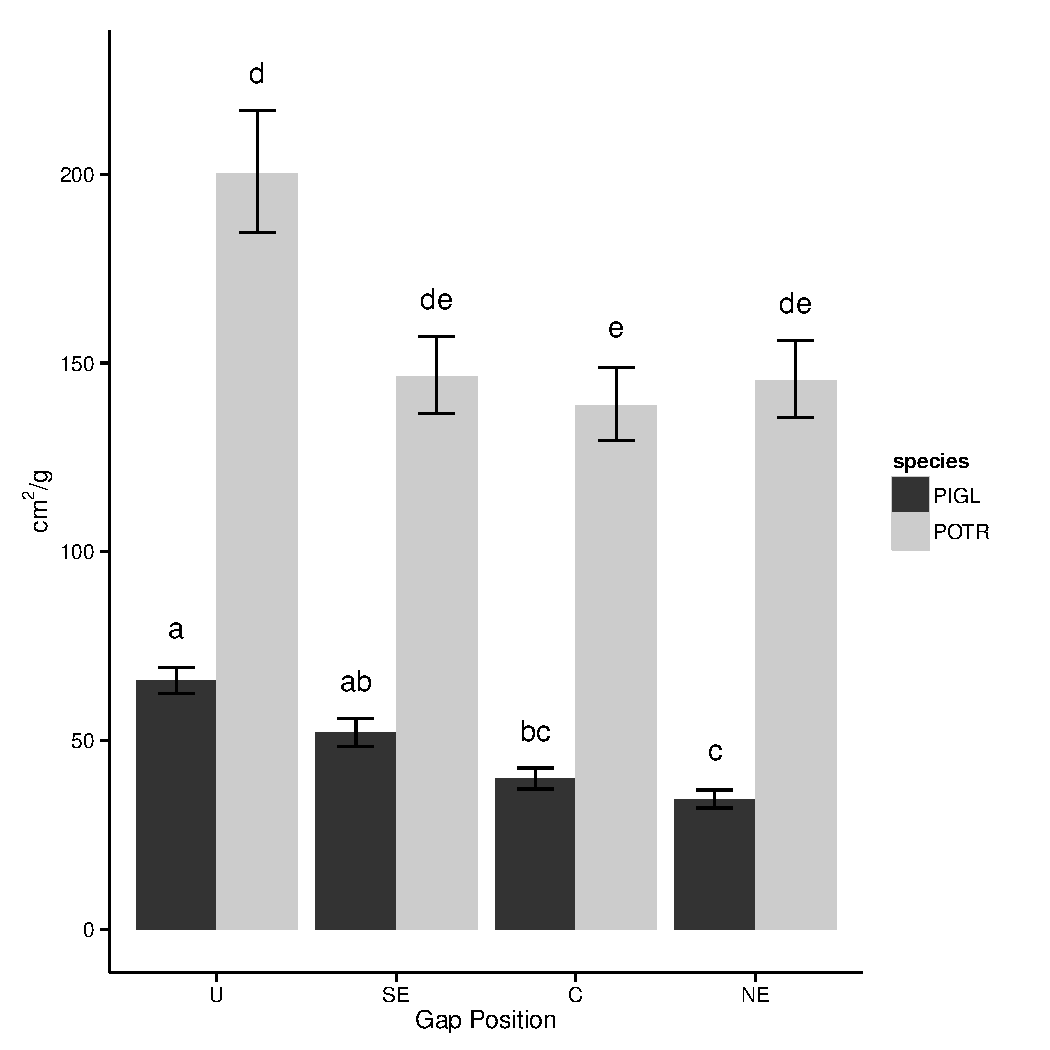
\includegraphics[width=\maxwidth]{figure/la_plot} 

\end{knitrout}




\end{multicols}
\begin{table}[t] % begins table
\centering
\subfloat[]{\scalebox{.6}{% latex table generated in R 3.0.1 by xtable 1.7-1 package
% Sat Aug 03 16:20:41 2013
\begin{tabular}{lrrrr}
  \hline
 & F & Df & Df.res & Pr($>$F) \\ 
  \hline
light & 4677.27 & 1 & 590 & 0.0000 \\ 
  species & 724.10 & 1 & 187 & 0.0000 \\ 
  gappos & 0.20 & 4 & 10 & 0.9312 \\ 
  vegtrt & 0.02 & 1 & 1 & 0.9152 \\ 
  light:species & 489.95 & 1 & 597 & 0.0000 \\ 
  light:gappos & 33.87 & 4 & 591 & 0.0000 \\ 
  species:gappos & 20.97 & 4 & 198 & 0.0000 \\ 
  light:vegtrt & 29.72 & 1 & 592 & 0.0000 \\ 
  species:vegtrt & 15.90 & 1 & 145 & 0.0001 \\ 
  gappos:vegtrt & 0.56 & 4 & 10 & 0.6941 \\ 
  light:species:gappos & 2.98 & 4 & 598 & 0.0188 \\ 
  light:species:vegtrt & 23.19 & 1 & 605 & 0.0000 \\ 
  light:gappos:vegtrt & 8.99 & 4 & 594 & 0.0000 \\ 
  species:gappos:vegtrt & 2.96 & 4 & 82 & 0.0244 \\ 
  light:species:gappos:vegtrt & 3.71 & 4 & 607 & 0.0054 \\ 
   \hline
\end{tabular}
}}\quad
\subfloat[]{\scalebox{.6}{% latex table generated in R 3.0.1 by xtable 1.7-1 package
% Sat Aug 03 16:20:41 2013
\begin{tabular}{lrrrr}
  \hline
 & F & Df & Df.res & Pr($>$F) \\ 
  \hline
light & 11.03 & 1 & 565 & 0.0010 \\ 
  species & 339.02 & 1 & 180 & 0.0000 \\ 
  gappos & 1.37 & 4 & 9 & 0.3155 \\ 
  vegtrt & 0.00 & 1 & 2 & 0.9691 \\ 
  light:species & 6.37 & 1 & 568 & 0.0119 \\ 
  light:gappos & 6.67 & 4 & 565 & 0.0000 \\ 
  species:gappos & 3.43 & 4 & 175 & 0.0100 \\ 
  light:vegtrt & 1.70 & 1 & 566 & 0.1925 \\ 
  species:vegtrt & 0.83 & 1 & 90 & 0.3644 \\ 
  gappos:vegtrt & 2.35 & 4 & 9 & 0.1316 \\ 
  light:species:gappos & 0.65 & 4 & 569 & 0.6258 \\ 
  light:species:vegtrt & 0.14 & 1 & 572 & 0.7130 \\ 
  light:gappos:vegtrt & 3.55 & 4 & 567 & 0.0071 \\ 
  species:gappos:vegtrt & 1.02 & 4 & 79 & 0.4003 \\ 
  light:species:gappos:vegtrt & 3.55 & 4 & 572 & 0.0072 \\ 
   \hline
\end{tabular}
}}\quad
\subfloat[]{\scalebox{.6}{% latex table generated in R 3.0.1 by xtable 1.7-1 package
% Sat Aug 03 16:20:41 2013
\begin{tabular}{lrrrr}
  \hline
 & F & Df & Df.res & Pr($>$F) \\ 
  \hline
light & 71.45 & 1 & 565 & 0.0000 \\ 
  species & 384.61 & 1 & 189 & 0.0000 \\ 
  gappos & 0.52 & 4 & 10 & 0.7219 \\ 
  vegtrt & 0.00 & 1 & 2 & 0.9895 \\ 
  light:species & 6.14 & 1 & 568 & 0.0135 \\ 
  light:gappos & 11.77 & 4 & 566 & 0.0000 \\ 
  species:gappos & 3.54 & 4 & 193 & 0.0081 \\ 
  light:vegtrt & 0.35 & 1 & 566 & 0.5538 \\ 
  species:vegtrt & 0.10 & 1 & 168 & 0.7465 \\ 
  gappos:vegtrt & 0.31 & 4 & 10 & 0.8618 \\ 
  light:species:gappos & 3.49 & 4 & 569 & 0.0078 \\ 
  light:species:vegtrt & 0.85 & 1 & 572 & 0.3579 \\ 
  light:gappos:vegtrt & 0.68 & 4 & 567 & 0.6084 \\ 
  species:gappos:vegtrt & 1.07 & 4 & 77 & 0.3782 \\ 
  light:species:gappos:vegtrt & 1.11 & 4 & 573 & 0.3528 \\ 
   \hline
\end{tabular}
}}
\caption{Results from Analysis of Deviance on the effects of light level, species, gap position, and vegetation treatment on (a) photosythesis, (b) conductance, and (c) transpiration}
\end{table}

% latex table generated in R 3.0.1 by xtable 1.7-1 package
% Sat Aug 03 16:20:41 2013
\begin{table}[ht]
\centering
\begin{tabular}{rrrrrr}
  \hline
 & Block & Transect & Plot & Tree & Residual \\ 
  \hline
Photosynthesis & 0.17 & 0.00 & 0.12 & 0.04 & 0.13 \\ 
  Conductance & 0.00 & 0.00 & 0.00 & 0.01 & 0.00 \\ 
  Transpiration & 0.00 & 0.02 & 0.04 & 0.04 & 0.02 \\ 
   \hline
\end{tabular}
\caption{Estimated standard deviations of random effects within gas exchange models.} 
\end{table}


\begin{multicols}{2}

\subsection{Gas Exchange}
Analysis of deviance results for fixed effects in full gas exchange models are shown in Table 2, and estimates of standard deviations of random effects of experimental design factors are displayed in Table 3. Based on parameter estimates from the full models, there appeared to be a high degree of interaction between experimental factors in all three gas exchange models. Significant four-way interactions between light, species, gap position, and vegetation treatment were indicated by the photosynthesis ($p=$0.0054) and stomatal conductance ($p=$0.0072) models. Likewise, results from the transpiration model indicated a significant ($p=$0) three-way interaction between light level, species, and gap position. 

In addition to being difficult to meaningfully interpret, however, the prima facie statistical significance of such high order interactions may at least in part be an artifact of fitting complex models to relatively noisy data, particularly at low light levels, and therefore not entirely demonstrative of strong physiological signals. Even with this caution in mind, however, estimates of gas exchange rates based on post-hoc comparisons of marginal means for fixed effects show some clear differences in patterns of species gas exchange rates in response to experimental factors. 

\end{multicols}
\begin{knitrout}
\definecolor{shadecolor}{rgb}{0.969, 0.969, 0.969}\color{fgcolor}\begin{figure}[]

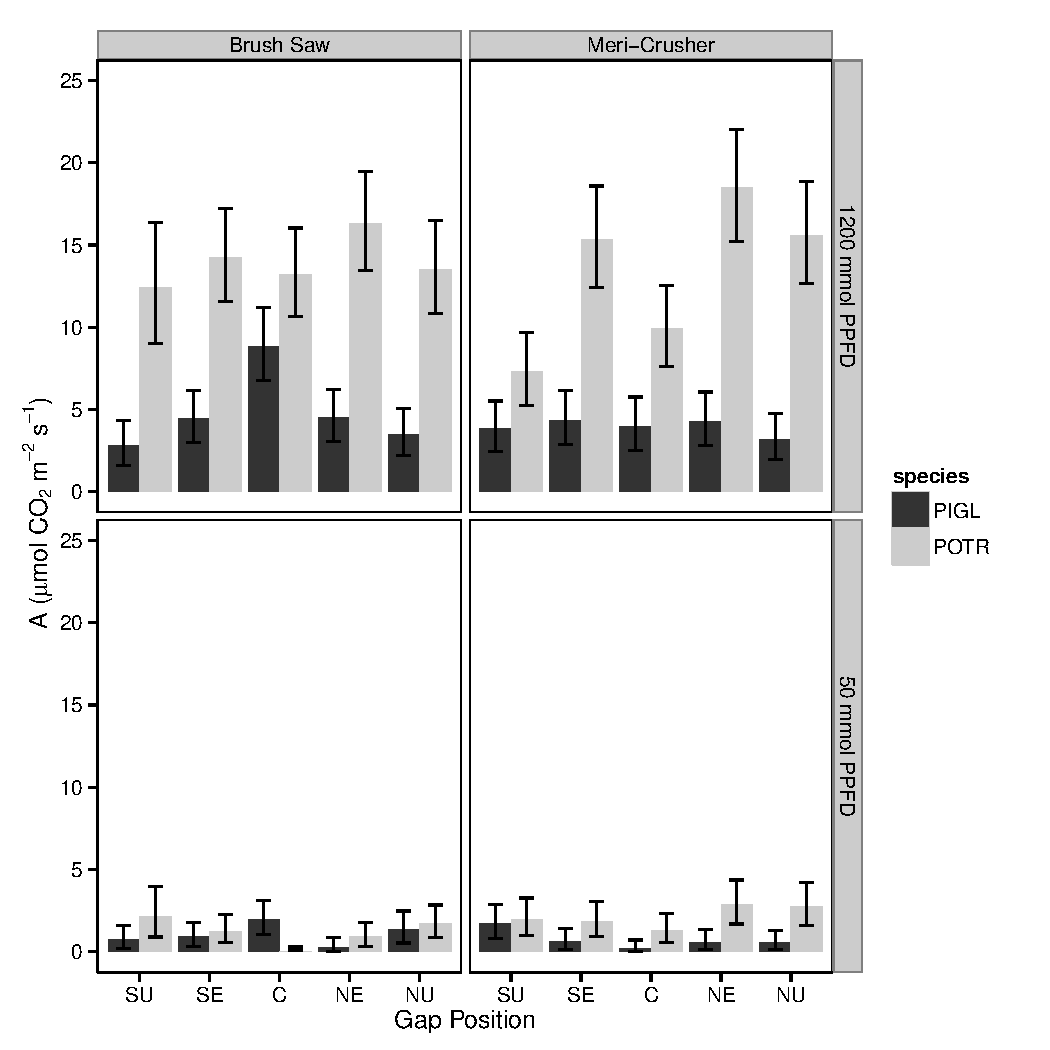
\includegraphics[width=\maxwidth]{figure/A_plot} \caption[Tukey's HSD pairwise comparisons of spruce (PIGL) and aspen (POTR) photosynthesis rates (marginal means $\pm$ SE) at differing light levels (1200 and 50 $\mu$mol m$^{-2}$ s$^{-1}$ PPFD), gap positions (SU = southern understory, SE = southern edge, C = center, NE = northern edge, NU = northern understory), and site prepapartion treatments (brush saw and Meri-crusher)]{Tukey's HSD pairwise comparisons of spruce (PIGL) and aspen (POTR) photosynthesis rates (marginal means $\pm$ SE) at differing light levels (1200 and 50 $\mu$mol m$^{-2}$ s$^{-1}$ PPFD), gap positions (SU = southern understory, SE = southern edge, C = center, NE = northern edge, NU = northern understory), and site prepapartion treatments (brush saw and Meri-crusher)\label{fig:A_plot}}
\end{figure}


\end{knitrout}

\begin{multicols}{2}

\subsubsection{Photosynthesis}

Post hoc comparisons of spruce and aspen photosythesis rates by light level, gap position, and vegetation treatment are presented in Figure 1. At low light levels there were some differences across the experiment, but these differences seemed largely idiosyncratic, not demonstrating a clear pattern. In low light levels both spruce and aspen appeared to be similarly limited, with rates in no gap position/vegetation treatment combination conclusively better than any other, and with neither species holding a clear advantage. By contrast, at full light aspen photosynthesis rates were both relatively constant and consistently higher than spruce, with the magnitude and significance of these differences between the two species varying based on site preparation treatment and gap position. 

In transects prepared with the brush saw treatment, recorded photosynthesis rates for aspen did not vary significantly by gap position, and were higher than spruce in all gap positions but the center. Spruce showed a more dynamic response, with photosynthesis rates significantly higher in the center than in surrounding gap positions, though with no detectable variation between the other gap positions. 

In transects prepared with the Meri-crusher treatment a wholly different pattern occured. Aspen photosynthesis rates were again higher than spruce in four of the five gap positions, but the location in which the two species did not vary significantly was instead the southern understory. Aspen photosynthesis rates were also variable rather than static from one gap position to another, with surprising differences between the center and northern edge gap positions, though no differences existed between the center and the southern edge, or the southern edge and the Because this variation is not easily interpretable physiologically, it should perhaps be treated as a statistical artifact rather than a definitive pattern.

\end{multicols}
\subsubsection{Stomatal Conductance}
\begin{knitrout}
\definecolor{shadecolor}{rgb}{0.969, 0.969, 0.969}\color{fgcolor}\begin{figure}[]

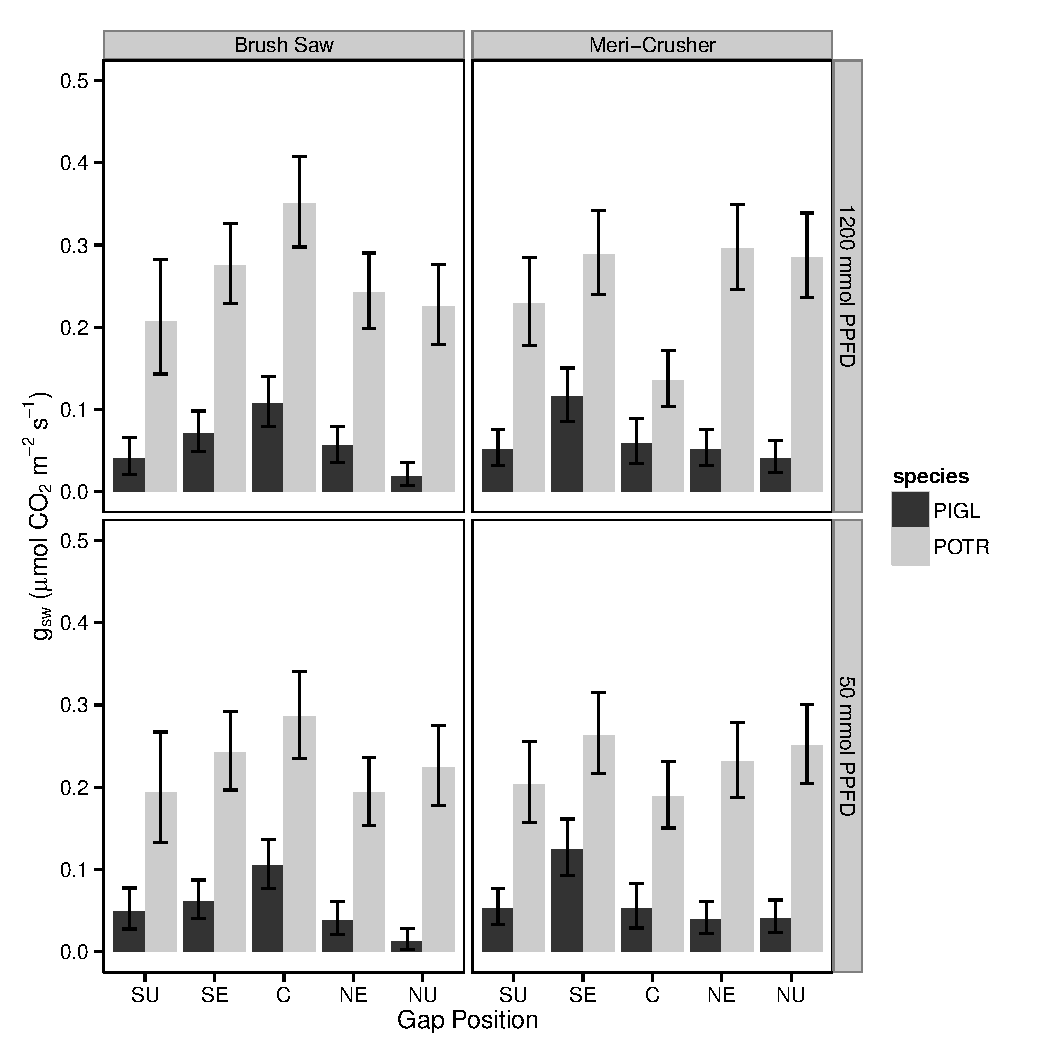
\includegraphics[width=\maxwidth]{figure/gs_plot} \caption[Marginal means $\pm$ SE of spruce (PIGL) and aspen (POTR) stomatal conductance to H$_2$O at differing light levels (1200 and 50 $\mu$mol m$^{-2}$ s$^{-1}$ PPFD), gap positions (SU = southern understory, SE = southern edge, C = center, NE = northern edge, NU = northern understory), and site prepapartion treatments (brush saw and Meri-crusher)]{Marginal means $\pm$ SE of spruce (PIGL) and aspen (POTR) stomatal conductance to H$_2$O at differing light levels (1200 and 50 $\mu$mol m$^{-2}$ s$^{-1}$ PPFD), gap positions (SU = southern understory, SE = southern edge, C = center, NE = northern edge, NU = northern understory), and site prepapartion treatments (brush saw and Meri-crusher)\label{fig:gs_plot}}
\end{figure}


\end{knitrout}

\begin{multicols}{2}

Post hoc comparisons of spruce and aspen stomatal conductance by light level, gap position, and vegetation treatment are presented in Figure 2. Aspen stomatal conductance was higher than that of spruce in all gap positions, regardless of changes in vegetation treatment or light level. Neither species showed distinct differences in stomatal conductance under changing light conditions, but aspen also showed very little variation across either gap environment or between site treatments. By contrast spruce showed distinctly different patterns in stomatal conductance rates between site preparation treatments, showing a more dynamic response to changes in gap position in the brush saw than the Meri-crusher transects. In brush sawn transects spruce stomatal conductance displayed an increasing pattern from the southern understory, peaking in the center of the gap and falling to very low levels in the northern understory. In contradistinction to this pattern, spruce stomatal conductance in Meri-crusher transects was highest in the southern edge of the gap, and did not vary significantly between all other gap positions.

\subsubsection{Transpiration}

Post hoc comparisons of spruce and aspen transpiration by light level and gap position are presented in Figure 3. Because of the non-significance of differences in vegetation treatment and interactions with vegetation treatment in the transpiration model, these factors were excluded from post-hoc testing. Transpiration was higher for aspen than spruce across all gap positions and both light levels, did not vary significantly by gap position within a given light level, and only varied between light levels at the northern edge of the harvest gap. Light level also made little difference in spruce transpiration rates. Similarly to other gas exchange measures, however, spruce showed a more dynamic response to changing gap position than aspen, with peak transpiration rates at the southern edge and center of the gap, and lowest transpiration rates in the two understory positions. 

\end{multicols}
\begin{knitrout}
\definecolor{shadecolor}{rgb}{0.969, 0.969, 0.969}\color{fgcolor}\begin{figure}[]

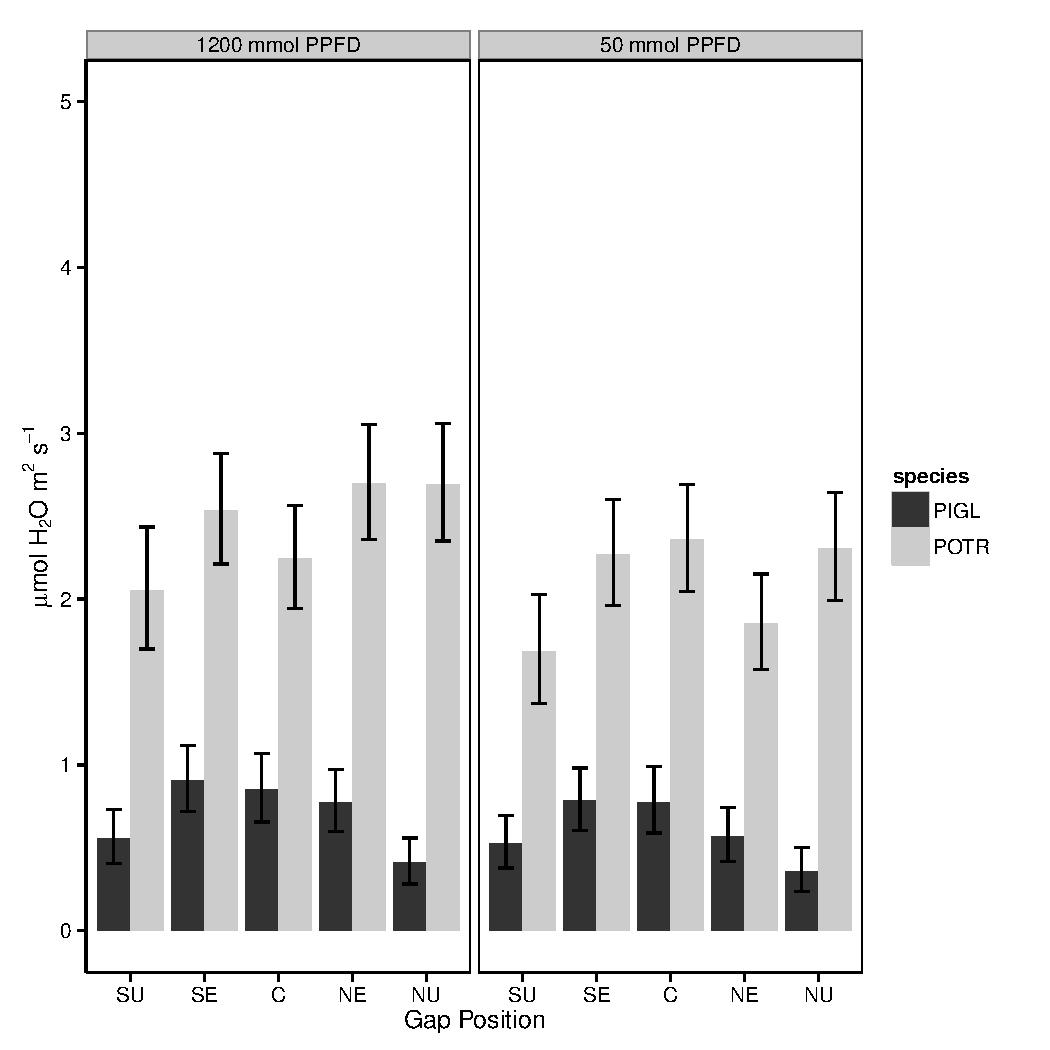
\includegraphics[width=\maxwidth]{figure/trmmol_plot} \caption[Results of Tukey's HSD pairwise comparisons between spruce and aspen transpiration rates by light level, gap position, and site preparation treatment]{Results of Tukey's HSD pairwise comparisons between spruce and aspen transpiration rates by light level, gap position, and site preparation treatment.\label{fig:trmmol.plot}}
\end{figure}


\end{knitrout}

\begin{multicols}{2}

\section{Discussion}
Our results suggest that spruce and aspen seedlings have distinctly different physiological responses to variations in post-harvest conditions within a forest gap environment. Overall, aspen LAW showed a more static response to differences in gap position, 

The comparatively lower photosynthesis 

Intensive site preparation treatments do not conclusively raise the gas exchange rates of aspen, but they possibly have the effect of shifting the ideal conditions for spruce growth from the gap center to the southern edge. This effect is possibly the result of lower soil moisture  

Determining what microenvironments may be most conducive to the competitive development of spruce within mixedwood spruce-aspen stands is crucial to designing silvicultural strategies that can successfully manage for these mixtures. We tested the differences in physiological ecology of spruce and aspen seedlings across a microenvironmental gradient within a linear gap, and also between site preparation treatments. Our results indicate that position within experimental linear gaps and the type of vegetation treatment applied to the site appear to be correlated to specific leaf area development in both spruce and aspen seedlings, though the pattern of responses of the two species to changes in the environmental gradient differ considerably. These differences in patterns of spruce and aspen response to gap environment and vegetation treatment reflect some of the mechanisms behind the successional niches of these two species. The ability of aspen to display a great deal of leaf area per unit weight largely without regard to the microclimatic variability of the harvest gap is characteristic of an early-successional species that is extremely competitive in a high-light, low moisture environment. This is doubly the case when the aspen is of sprout origin, for which moisture is likely less limiting than for released individuals. By contrast, spruce is a relatively shade tolerant species whose successional status in natural stands relies on persistence beneath aspen, with slower growth but greater longevity. 

\section{Citations}
\end{multicols}
\end{document}
